\section{Experiments}
\label{sec:experiments}

\subsection{Experimental Setup}
\label{subsec:setup}
% \paragraph*{Datasets and Benchmarks}
% We evaluate FlexTrack-V2 on 5 multimodal tracking benchmarks spanning three modality pairs: 
% RGB-Thermal (e.g., LasHeR~\cite{li2021lasher}, RGBT234~\cite{rgbt234}), 
% RGB-Depth (e.g., DepthTrack~\cite{depthtrack}, VOT-RGBD22\cite{vot2022}), 
% and RGB-Event (e.g., VisEvent~\cite{wang2023visevent}). 
% To validate robustness, we evaluate under both the standard \emph{complete-modality} setting and a \emph{missing-modality} protocol, where the auxiliary sensor drops out either randomly or in contiguous chunks.

\paragraph*{Datasets and Benchmarks}
We evaluate FlexTrack-V2 on five multimodal tracking benchmarks spanning three modality pairs: \emph{RGB-Thermal}, \emph{RGB-Depth}, and \emph{RGB-Event}. These benchmarks collectively cover a diverse range of real-world challenges including low illumination, fast motion, occlusion, and background clutter—scenarios where the complementary sensor provides critical information beyond RGB. To validate robustness under realistic sensor degradation, we evaluate under both the standard \emph{complete-modality} setting and a \emph{missing-modality} protocol, where the auxiliary sensor drops out either randomly or in contiguous chunks.

% \begin{itemize}
For RGB-Thermal, we employ two widely adopted RGB-T datasets. LasHeR\cite{li2021lasher} comprises 1,224 spatially aligned RGB-thermal video pairs with over 730K frame pairs in total. It covers 32 object categories and is annotated with 19 challenging attributes captured from multiple imaging platforms across diverse seasons, weather conditions, and day-night cycles. LasHeR provides dedicated training and evaluation splits, serving as the primary benchmark for large-scale RGBT tracking. RGBT234\cite{rgbt234} contains 234 highly aligned RGB-T video pairs with 233.8K frames, spanning 22 object categories and 12 attributes with per-frame occlusion annotation. Recorded from a moving camera platform, RGBT234 introduces additional challenges such as thermal crossover and camera motion, complementing the attribute distribution of LasHeR. Together, the two benchmarks enable comprehensive evaluation over both large-scale and attribute-rich settings.
    
For RGB-Depth, we evaluate on DepthTrack\cite{depthtrack} and VOT-RGBD22\cite{vot2022}. DepthTrack is the largest and most diverse RGBD tracking dataset, consisting of 200 sequences (150 training, 50 test) totaling 294.6K frames across 40 scene types and 90 object categories. Designed as a long-term tracking benchmark, DepthTrack requires trackers to detect target disappearance and re-identify targets upon reappearance. VOT-RGBD22 provides a complementary short-term evaluation perspective. It comprises 127 sequences drawn from the CDTB\cite{lukezic2019cdtb} and DepthTrack test splits, converted to the anchor-based short-term protocol adopted by the VOT2022 challenge. The pairing of long-term and short-term benchmarks yields a thorough assessment of RGBD tracking performance.
    
For RGB-Event, we adopt VisEvent\cite{wang2023visevent}, a large-scale realistic visible-event tracking benchmark. It contains 820 video pairs with 371,128 frames in total, captured at a resolution of $346 \times 260$ using a single Dynamic Vision Sensor that simultaneously outputs temporally and spatially aligned RGB frames and event streams. VisEvent covers 18 target categories (primarily pedestrians and vehicles in traffic scenes, supplemented by indoor scenarios) and is annotated with 17 attributes that encompass both conventional tracking challenges like occlusion, scale variation, and camera motion, as well as event-specific ones including fast motion, motion blur, and no-motion that arise from the unique sensing characteristics of event cameras.
% \end{itemize}

\paragraph*{Evaluation Metrics}
We follow the standard evaluation protocols established by each benchmark, which vary across modality pairs to reflect the distinct nature of each tracking task.

\begin{itemize}
    \item RGB-Thermal metrics. For LasHeR, performance is measured by Precision Rate (PR) and Success Rate (SR). 
    PR computes the percentage of frames in which the center location error between the predicted and ground-truth bounding boxes falls within a threshold. 
    SR is defined as the percentage of frames whose intersection-over-union exceeds a certain threshold. 
    For RGBT234, we report the Maximum Precision Rate (MPR) and Maximum Success Rate (MSR). 
    MPR and MSR respectively denote the precision and success rates computed from the per-frame smaller center error and larger overlap between the two modalities.
    \item RGB-Depth metrics. 
    For DepthTrack, performance is quantified by three complementary measures: Precision (Pr), Recall (Re), and F-score. Precision (Pr) measures the bounding-box overlap accuracy on frames where the target is labeled visible, while Recall (Re) measures the tracker's ability to correctly identify those visible frames given its self-reported confidence score. F-score, the harmonic mean of Pr and Re, serves as the primary ranking metric and is reported at the per-tracker confidence threshold that maximizes it.
    For VOT-RGBD22, the anchor-based protocol initializes the tracker at multiple anchor points per sequence and runs it over the resulting sub-sequences without reset. Performance is evaluated by Expected Average Overlap (EAO), Accuracy (Acc.), and Robustness (Rob.). Accuracy (Acc.) is the average overlap over sub-sequences that are successfully tracked and Robustness (Rob.) is the percentage of sub-sequences completed without failure. Expected Average Overlap (EAO) combines Accuracy and Robustness into a single metric that estimates the expected overlap a tracker would attain on a typical short-term sequence, and serves as the primary ranking measure.
    \item RGB-Event metrics. For VisEvent, we report Precision Rate (PR) and Success Rate (SR), computed identically to LasHeR.
\end{itemize}

\paragraph*{Implementation Details}
XXX.

For training, XXX.

For testing, XXX.


\subsection{Main Results}
\label{subsec:main_results}
% 1) Complete Modalities Parity
% 2) Missing Modalities Superiority
We compare FlexTrack-V2 against state-of-the-art multimodal trackers, including our conference baseline FlexTrack-V1~\cite{tan2025you}. 

As shown in Table~\ref{tab-sota-miss}, under complete modalities, FlexTrack-V2 matches or slightly exceeds the performance of prior methods, validating that our generative pathway does not compromise intact data. Under the missing-modality regime, FlexTrack-V2 demonstrates substantial gains. Trackers that rely on passive masking or zero-padding degrade sharply, whereas our BMR-HMoE maintains stable tracking by hallucinating the missing auxiliary features. 

\begin{table*}[t]
\caption{SOTA comparison on $\mathrm{DepthTrack}$ \cite{depthtrack} and VOT-RGBD22~\cite{vot2022} for RGB-Depth, $\mathrm{LasHeR}$\cite{li2021lasher} and $\mathrm{RGBT234}$\cite{rgbt234} for RGB-Thermal, and $\mathrm{VisEvent}$\cite{wang2023visevent} for RGB-Event. The best and second methods are labeled with \textbf{bold} and \underline{underline} styles.}
\label{tab-sota-miss}
\centering
\setlength{\tabcolsep}{3mm} % 设置列间距
\small % 设置字体大小
\begin{tabular}{l|ccc|ccc|cc|cc|cc}
\toprule
\multirow{2}{*}{Method} 
& \multicolumn{3}{c|}{DepthTrack~\cite{depthtrack}} 
& \multicolumn{3}{c|}{VOT-RGBD22~\cite{vot2022}}
& \multicolumn{2}{c|}{LasHeR~\cite{li2021lasher}} 
& \multicolumn{2}{c|}{RGBT234~\cite{rgbt234}} 
& \multicolumn{2}{c}{VisEvent~\cite{wang2023visevent}} \\
\cmidrule(lr){2-4} \cmidrule(lr){5-7} \cmidrule(lr){8-9} \cmidrule(lr){10-11} \cmidrule(lr){12-13}
& F-score & Re & Pr 
& EAO & Acc.& Rob.
& PR & SR 
& MPR & MSR 
& PR & SR \\
\midrule
SiamM-Ds~\cite{VOT2019}
& 33.6 & 26.4 & 46.3 &  -   &  -   &  -   &  -   &  -   &  -   &  -   &  -   &  -   \\
SiamMask\_E~\cite{SiamMask}
&  -   &  -   &  -   &  -   &  -   &  -   &  -   &  -   &  -   &  -   & 56.2 & 36.9 \\
% Siam-LTD~\cite{vot2020}
% & 37.6 & 34.2 & 41.8 &  -   &  -   &  -   &  -   &  -   &  -   &  -   &  -   &  -   \\
ATCAIS~\cite{vot2020}
& 47.6 & 45.5 & 50.0 & 55.9 & 76.1 & 73.9 &  -   &  -   &  -   &  -   &  -   &  -   \\
FANet~\cite{fanet}
&  -   &  -   &  -   &  -   &  -   &  -   & 44.1 & 30.9 & 78.7 & 55.3 &  -   &  -   \\
SiamBAN\_E~\cite{siamban}
&  -   &  -   &  -   &  -   &  -   &  -   &  -   &  -   &  -   &  -   & 59.1 & 40.5\\
GLGS-D~\cite{vot2020}
& 45.3 & 36.9 & 58.4 &  -   &  -   &  -   &  -   &  -   &  -   &  -   &  -   &  -   \\
ATOM~\cite{atom}
&  -   &  -   &  -   & 50.5 & 59.8 & 68.8 &  -   &  -   &  -   &  -   &  -   &  -   \\

SiamCar\_E~\cite{Stark}
&  -   &  -   &  -   &  -   &  -   &  -   &  -   &  -   &  -   &  -   & 59.9 & 42.0\\
DiMP~\cite{dimp}
&  -   &  -   &  -   & 54.3 & 70.3 & 73.1 &  -   &  -   &  -   &  -   &  -   &  -   \\
LTDSEd~\cite{VOT2019}
& 40.5 & 38.2 & 43.0 &  -   &  -   &  -   &  -   &  -   &  -   &  -   &  -   &  -   \\

MaCNet~\cite{macnet}
&  -   &  -   &  -   &  -   &  -   &  -   &  -   &  -   & 79.0 & 55.4 &  -   &  -   \\
DAL~\cite{dal}
& 42.9 & 36.9 & 51.2 &  -   &  -   &  -   &  -   &  -   &  -   &  -   &  -   &  -   \\
CAT~\cite{cat}
&  -   &  -   &  -   &  -   &  -   &  -   & 45.0 & 31.4 & 80.4 & 56.1 &  -   &  -   \\
DMTrack~\cite{vot2022}
&  -   &  -   &  -   & 65.8 & 75.8 & 85.1 &  -   &  -   &  -   &  -   &  -   &  -   \\
DDiMP~\cite{vot2020}
& 48.5 & 56.9 & 50.3 &  -   &  -   &  -   &  -   &  -   &  -   &  -   &  -   &  -   \\
% ATOM\_E~\cite{atom}
% &  -   &  -   &  -   &  -   &  -   &  -   &  -   &  -   &  -   &  -   & 60.8 & 41.2\\
MDNet\_E~\cite{MDNet}
&  -   &  -   &  -   &  -   &  -   &  -   &  -   &  -   &  -   &  -   & 66.1 & 42.6\\
ProTrack~\cite{protrack} 
& 57.8 & 57.3 & 58.3 & 65.1 & 80.1 & 80.2 & 53.8 & 42.0 & 79.5 & 59.9 & 63.2 & 47.1\\
VITAL\_E~\cite{VITAL}
&  -   &  -   &  -   &  -   &  -   &  -   &  -   &  -   &  -   &  -   & 64.9 & 41.5\\
% PrDiMP\_E~\cite{PrDiMP}
% &  -   &  -   &  -   &  -   &  -   &  -   &  -   &  -   &  -   &  -   & 64.4 & 45.3\\
LTMU-B~\cite{LTMU}
& 46.0 & 41.7 & 51.2 &  -   &  -   &  -   &  -   &  -   &  -   &  -   &  -   &  -   \\
OSTrack~\cite{ostrack}
& 52.9 & 52.2 & 53.6 & 67.6 & 80.3 & 83.3 & 51.5 & 41.2 & 72.9 & 54.9 & 69.5 & 53.4 \\
LTMU\_E~\cite{LTMU}
&  -   &  -   &  -   &  -   &  -   &  -   &  -   &  -   &  -   &  -   & 65.5 & 45.9\\
% TransT\_E~\cite{transt}
% &  -   &  -   &  -   &  -   &  -   &  -   &  -   &  -   &  -   &  -   & 65.0 & 47.4\\
MCITrack~\cite{mcitrack} 
& 53.8 & 54.9 & 52.7 & 74.3 & 82.3 & 90.6 & 64.2 & 50.2 & 79.1 & 60.4 & 69.7 & 53.3\\
SiamRCNN\_E~\cite{SiamRCNN}
&  -   &  -   &  -   &  -   &  -   &  -   &  -   &  -   &  -   &  -   & 65.9 & 49.9\\
JMMAC~\cite{jmmac}
&  -   &  -   &  -   &  -   &  -   &  -   &  -   &  -   & 79.0 & 57.3 &  -   &  -   \\

ViPT~\cite{vipt} 
& 59.4 & 59.6 & 59.2 & 72.1 & 81.5 & 87.1 & 65.1 & 52.5 & 83.5 & 61.7 & 75.8 & 59.2\\
CMPP~\cite{cmpp}
&  -   &  -   &  -   &  -   &  -   &  -   &  -   &  -   & 82.3 & 57.5 &  -   &  -   \\
APFNet~\cite{apfnet}
&  -   &  -   &  -   &  -   &  -   &  -   & 50.0 & 36.2 & 82.7 & 57.9 &  -   &  -   \\
% CA3DMS~\cite{ca3dms}
% & 22.3 & 22.8 & 21.8 &  -   &  -   &  -   &  -   &  -   &  -   &  -   &  -   &  -   \\


DeT~\cite{depthtrack}
& 53.2 & 50.6 & 56.0 & 65.7 & 76.0 & 84.5 &  -   &  -   &  -   &  -   &  -   &  -   \\
SPT~\cite{rgbd1k}
& 53.8 & 54.9 & 52.7 & 65.1 & 79.8 & 85.1 &  -   &  -   &  -   &  -   &  -   &  -   \\
UnTrack~\cite{untrack} 
& 61.0 & 60.8 & 61.1 & 72.1 & 82.0 & 86.9 & 64.6 & 51.3 & 84.2 & 62.5 & 75.5 & 58.9\\
SBT-RGBD~\cite{sbt}
&  -   &  -   &  -   & 70.8 & 80.9 & 86.4 &  -   &  -   &  -   &  -   &  -   &  -   \\
SDSTrack~\cite{hou2024sdstrack} 
& 61.4 & 60.9 & 61.9 & 72.8 & 81.2 & 88.3 & 66.5 & 53.1 & 84.8 & 62.5 & 76.7 & 59.7\\
OneTracker~\cite{hong2024onetracker} 
& 60.9 & 60.4 & 60.7 & 72.7 & 81.9 & 87.2 & 67.2 & 53.8 & 85.7 & 64.2 & 76.7 & 60.8\\
SUTrack~\cite{chen2024sutrack} 
& 65.1 & \underline{65.7} & 64.5 & 76.5 & 82.8 & 91.8 & 74.5 & 59.5 & 92.2 & \underline{69.5} & 79.9 & 62.7\\
STTrack~\cite{sttrack} 
& 63.3 & 63.4 & 63.2 & 77.6 & 82.5 & 93.7 & \underline{76.0} & 60.3 & 89.8 & 66.7 & 78.6 & 61.9\\
FlexTrack 
& \underline{67.0} & \textbf{66.9} & \textbf{67.1} & \underline{78.0} & \underline{83.8} & \underline{93.1} & \textbf{77.3} & \textbf{62.0} & \underline{92.7} & \textbf{69.9} & \textbf{81.3} & \textbf{64.1}\\

\midrule

\textbf{FlexTrackV2 (ours)}
& \textbf{67.8} & \textbf{69.3} & \underline{66.4} & \textbf{78.4}  & \textbf{83.9}  & \textbf{93.9} & \textbf{77.3} & \underline{61.9} & \textbf{93.4} & \textbf{69.9} & \underline{81.2} & \underline{64.0}\\

\bottomrule
\end{tabular}
\end{table*}





\begin{table*}[t]
\caption{SOTA comparison on $\mathrm{DepthTrack}_{miss}$ \cite{depthtrack} for RGB-Depth, $\mathrm{LasHeR}_{miss}$\cite{li2021lasher} and $\mathrm{RGBT234}_{miss}$\cite{rgbt234} for RGB-Thermal, and $\mathrm{VisEvent}_{miss}$\cite{wang2023visevent} for RGB-Event. The best and second methods are labeled with \textbf{bold} and \underline{underline} styles.}
\label{tab-sota-miss}
\centering
\setlength{\tabcolsep}{3mm} % 设置列间距
\small % 设置字体大小
\begin{tabular}{l|ccc|cc|cc|cc}
\toprule
\multirow{2}{*}{Method} 
& \multicolumn{3}{c|}{DepthTrack$_{miss}$~\cite{depthtrack}} 
& \multicolumn{2}{c|}{LasHeR$_{miss}$~\cite{li2021lasher}} 
& \multicolumn{2}{c|}{RGBT234$_{miss}$~\cite{rgbt234}} 
& \multicolumn{2}{c}{VisEvent$_{miss}$~\cite{wang2023visevent}} \\
\cline{2-4} \cline{5-6} \cline{7-8} \cline{9-10}
& F-score & Re & Pr 
& PR & SR 
& MPR & MSR 
& PR & SR \\
\midrule

MCITrack~\cite{mcitrack} 
& 49.7 & 42.9 & 59.1 & 34.2 & 40.0 & 53.6 & 40.9 & 49.9 & 36.5 \\
ViPT~\cite{vipt} 
& 44.4 & 40.5 & 46.6 & 40.1 & 34.0 & 52.4 & 39.4 & 57.2 & 43.2 \\
IPT~\cite{ipt} 
& - & - & - & 61.7 & 46.4 & 82.0 & 59.4 & - & - \\
SDSTrack~\cite{hou2024sdstrack} 
& 46.7 & 42.0 & 52.7 & 52.5 & 43.1 & 67.0 & 48.8 & 62.6 & 46.9 \\
SeqTrackv2~\cite{seqtrack} 
& 45.0 & 40.9 & 50.0 & 50.0 & 39.9 & 70.8 & 49.9 & 57.6 & 43.1 \\
SUTrack~\cite{chen2024sutrack} 
& 49.5 & 47.3 & 51.9 & 58.3 & 47.6 & 82.0 & 60.8 & 66.6 & 50.5 \\
STTrack \cite{sttrack} 
& 49.9 & {48.8} & 51.0 & 54.5 & 44.9 & 73.8 & 54.2 & 65.5 & 49.7 \\
FlexTrack & \underline{57.8} & \underline{56.1} & \textbf{59.6} & \underline{65.1} & \underline{52.3} & \underline{84.1} & \underline{62.6} & \underline{72.8} & \underline{55.0} \\

\midrule

\textbf{FlexTrackV2 (ours)}
& \textbf{58.8} & \textbf{60.1} & \underline{57.5} & \textbf{67.6} & \textbf{54.4} & \textbf{85.6} & \textbf{62.9} & \textbf{75.1} & \textbf{56.9}\\

\bottomrule
\end{tabular}
\end{table*}


% \begin{table*}[t]
% \caption{SOTA comparison on $\mathrm{DepthTrack}$ \cite{depthtrack} and VOT-RGBD22~\cite{vot2022} for RGB-Depth, $\mathrm{LasHeR}$\cite{li2021lasher} and $\mathrm{RGBT234}$\cite{rgbt234} for RGB-Thermal, and $\mathrm{VisEvent}$\cite{wang2023visevent} for RGB-Event. The best and second methods are labeled with {bold} and {underline} styles.}
% \label{tab-sota-miss}
% \centering
% \setlength{\tabcolsep}{3mm} % 设置列间距
% \small % 设置字体大小
% \begin{tabular}{l|ccc|ccc|cc|cc|cc}
% \toprule
% \multirow{2}{*}{Method} 
% & \multicolumn{3}{c|}{DepthTrack~\cite{depthtrack}} 
% & \multicolumn{3}{c|}{VOT-RGBD22~\cite{vot2022}}
% & \multicolumn{2}{c|}{LasHeR~\cite{li2021lasher}} 
% & \multicolumn{2}{c|}{RGBT234~\cite{rgbt234}} 
% & \multicolumn{2}{c}{VisEvent~\cite{wang2023visevent}} \\
% \cmidrule(lr){2-4} \cmidrule(lr){5-7} \cmidrule(lr){8-9} \cmidrule(lr){10-11} \cmidrule(lr){12-13}
% & F-score & Re & Pr 
% & EAO & Acc.& Rob.
% & P & AUC 
% & MPR & MSR 
% & P & AUC \\
% \midrule

% FANet~\cite{fanet}
% &  -   &  -   &  -   &  -   &  -   &  -   & 44.1 & 30.9 & 78.7 & 55.3 &  -   &  -   \\
% CAT~\cite{cat}
% &  -   &  -   &  -   &  -   &  -   &  -   & 45.0 & 31.4 & 80.4 & 56.1 &  -   &  -   \\
% APFNet~\cite{apfnet}
% &  -   &  -   &  -   &  -   &  -   &  -   & 50.0 & 36.2 & 82.7 & 57.9 &  -   &  -   \\
% ATCAIS~\cite{vot2020}
% & 47.6 & 45.5 & 50.0 & 55.9 & 76.1 & 73.9 &  -   &  -   &  -   &  -   &  -   &  -   \\
% DeT~\cite{depthtrack}
% & 53.2 & 50.6 & 56.0 & 65.7 & 76.0 & 84.5 &  -   &  -   &  -   &  -   &  -   &  -   \\
% SPT~\cite{rgbd1k}
% & 53.8 & 54.9 & 52.7 & 65.1 & 79.8 & 85.1 &  -   &  -   &  -   &  -   &  -   &  -   \\
% OSTrack~\cite{ostrack}
% & 52.9 & 52.2 & 53.6 & 67.6 & 80.3 & 83.3 & 51.5 & 41.2 & 72.9 & 54.9 & 69.5 & 53.4 \\
% MCITrack~\cite{mcitrack} 
% & 53.8 & 54.9 & 52.7 & 74.3 & 82.3 & 90.6 & 64.2 & 50.2 & 79.1 & 60.4 & 69.7 & 53.3\\
% ProTrack~\cite{protrack} 
% & 57.8 & 57.3 & 58.3 & 65.1 & 80.1 & 80.2 & 53.8 & 42.0 & 79.5 & 59.9 & 63.2 & 47.1\\
% ViPT~\cite{vipt} 
% & 59.4 & 59.6 & 59.2 & 72.1 & 81.5 & 87.1 & 65.1 & 52.5 & 83.5 & 61.7 & 75.8 & 59.2\\
% UnTrack~\cite{untrack} 
% & 61.0 & 60.8 & 61.1 & 72.1 & 82.0 & 86.9 & 64.6 & 51.3 & 84.2 & 62.5 & 75.5 & 58.9\\
% SDSTrack~\cite{hou2024sdstrack} 
% & 61.4 & 60.9 & 61.9 & 72.8 & 81.2 & 88.3 & 66.5 & 53.1 & 84.8 & 62.5 & 76.7 & 59.7\\
% OneTracker~\cite{hong2024onetracker} 
% & 60.9 & 60.4 & 60.7 & 72.7 & 81.9 & 87.2 & 67.2 & 53.8 & 85.7 & 64.2 & 76.7 & 60.8\\
% SUTrack~\cite{chen2024sutrack} 
% & 65.1 & \underline{65.7} & 64.5 & 76.5 & 82.8 & 91.8 & 74.5 & 59.5 & 92.2 & \underline{69.5} & 79.9 & 62.7\\
% STTrack~\cite{sttrack} 
% & 63.3 & 63.4 & 63.2 & 77.6 & 82.5 & 93.7 & \underline{76.0} & 60.3 & 89.8 & 66.7 & 78.6 & 61.9\\
% FlexTrack 
% & \underline{67.0} & \textbf{66.9} & \textbf{67.1} & \underline{78.0} & \underline{83.8} & \underline{93.1} & \textbf{77.3} & \textbf{62.0} & \underline{92.7} & \textbf{69.9} & \textbf{81.4} & \textbf{64.1}\\

% \midrule

% \textbf{FlexTrackV2 (ours)}
% & \textbf{67.1} & \textbf{66.9} & \underline{67.0} & \textbf{78.4}  & \textbf{83.9}  & \textbf{93.9}  & \textbf{77.3} & \underline{61.9} & \textbf{93.4} & \textbf{69.9} & \underline{81.2} & \underline{64.0}\\

% \bottomrule
% \end{tabular}
% \end{table*}

\subsection{Ablation Studies}
\label{subsec:ablation}
% To understand the contribution of each module, we run ablation studies using the RGB-T LasHeR dataset under a 30\% missing rate.

% \begin{table}[ht]
% \caption{Effectiveness of the BMR module on LasHeR (30\% missing rate). Active compensation (BMR) yields the highest success and precision rates compared to passive strategies.}
% \label{tab:ablation_modules}
% \centering
% \small
% \begin{tabular}{lccc}
% \toprule
% Variant & PR $\uparrow$ & NPR $\uparrow$ & SR $\uparrow$ \\
% \midrule
% Zero-padding & 45.2 & 40.1 & 35.8 \\
% Last-frame repetition & 48.7 & 43.5 & 39.2 \\
% Passive masking (FlexTrack-V1) & 52.4 & 48.0 & 42.1 \\
% \rowcolor{gray!10} \textbf{BMR-HMoE (Ours)} & \textbf{58.9} & \textbf{55.2} & \textbf{49.7} \\
% \bottomrule
% \end{tabular}
% \end{table}


% Ablation 1: The BMR Module
\paragraph*{Effectiveness of Active Compensation (BMR)}
\begin{table}[ht]
\caption{Impact of Feature Hallucination on LasHeR$_\text{miss}$ and DepthTrack$_\text{miss}$.}
\label{tab:ablation_cma}
\setlength{\tabcolsep}{1.5mm}
\centering
\small
\scalebox{0.85}{
\begin{tabular}{c|ccccc}
\toprule
\multirow{2}{*}{Experimental Setting} & \multicolumn{2}{c}{LasHeR\cite{li2021lasher}} & \multicolumn{3}{c}{DepthTrack\cite{depthtrack}} \\
\cline{2-3} \cline{4-6} & PR & SR & F-score & Re & Pr \\
\midrule
w/o BMR & 67.4 & 54.0 & 57.4 & 58.6 & 56.1 \\
+ Feature Hal. & 66.1$^{\textcolor{red!90!black}{\downarrow{1.3}}}$ & 53.4$^{\textcolor{red!90!black}{\downarrow{0.6}}}$ & 56.0$^{\textcolor{red!90!black}{\downarrow{1.4}}}$ & 57.3$^{\textcolor{red!90!black}{\downarrow{1.3}}}$ & 54.8$^{\textcolor{red!90!black}{\downarrow{1.3}}}$ \\
+ Recon. Loss & \textbf{67.6$^{\textcolor{green!80!black}{\uparrow{0.2}}}$} & \textbf{54.4$^{\textcolor{green!80!black}{\uparrow{0.4}}}$} & \textbf{58.8$^{\textcolor{green!80!black}{\uparrow{1.4}}}$} & \textbf{60.1$^{\textcolor{green!80!black}{\uparrow{1.5}}}$} & \textbf{57.5$^{\textcolor{green!80!black}{\uparrow{1.4}}}$} \\ 
\bottomrule
\end{tabular}
}
\end{table}




\begin{table}[ht]
\caption{Impact of Fusion Directionality and Orthogonal Regularization on LasHeR.}
\label{tab:ablation_cma}
\setlength{\tabcolsep}{1.1mm}
\centering
\small
\scalebox{0.85}{
\begin{tabular}{cccc|cccc|cc}
\toprule
\multicolumn{3}{c}{Fusion Directionality} & \multirow{2}{*}{Ortho. Reg.} & \multirow{2}{*}{PR$_\text{full}$} & \multirow{2}{*}{PR$_\text{miss}$} & \multirow{2}{*}{SR$_\text{full}$} & \multirow{2}{*}{SR$_\text{miss}$} & \multirow{2}{*}{\textcolor{gray}{$\Delta_\text{PR}$}} & \multirow{2}{*}{\textcolor{gray}{$\Delta_\text{SR}$}} \\
\cline{1-3}
R$\rightarrow$A & A$\rightarrow$R & R$\leftrightarrow$A & & & & & & & \\
\midrule
\checkmark & & & &  &  &  & \\
\checkmark & & & \checkmark & 76.0 & 67.3 & 60.9 & 54.2 & \textcolor{gray}{-8.7} & \textcolor{gray}{-6.7}\\
\midrule
& \checkmark & & & 76.4 & 66.1 & 61.3 & 53.2 & \textcolor{lightgray}{-10.3} & \textcolor{lightgray}{-8.1}\\
& \checkmark & & \checkmark & 76.0 & 66.8 & 60.9 & 53.8 & \textcolor{gray}{-9.2} & \textcolor{gray}{-7.1}\\
\midrule
& & \checkmark & & 76.9 & 65.9 & 61.6 & 53.1 & \textcolor{lightgray}{-11.0} & \textcolor{lightgray}{-8.5}\\
& & \checkmark & \checkmark & \textbf{77.3} & \textbf{67.6} & \textbf{61.9} & \textbf{54.4}& \textcolor{gray}{-9.7} & \textcolor{gray}{-7.5}\\
\bottomrule
\end{tabular}
}
\end{table}



\paragraph*{Effectiveness of Curriculum Missing Augmentation and Self-Distillation}
\begin{table}[ht]
\caption{Impact of Curriculum Missing Augmentation (CMA) and Self-Distillation on LasHeR}
\label{tab:ablation_cma}
\centering
\small
\scalebox{0.9}{
\begin{tabular}{ccc|cccc}
\toprule
\multicolumn{2}{c}{Curriculum} & \multirow{2}{*}{$\mathcal{L}_{\text{dist}}$} & \multirow{2}{*}{PR$_\text{full}$} & \multirow{2}{*}{PR$_\text{miss}$} & \multirow{2}{*}{SR$_\text{full}$} & \multirow{2}{*}{SR$_\text{miss}$} \\
\cline{1-2}
Fixed 20\% & Annealed & & & & \\
\midrule
\checkmark & & &  &  &  & \\
\checkmark & & \checkmark & 76.3 & 66.5 & 61.3 & 53.7 \\
& \checkmark & & 76.9 & 66.9 & 61.8 & 53.9 \\
& \checkmark & \checkmark & \textbf{77.3} & \textbf{67.6} & \textbf{61.9} & \textbf{54.4} \\
\bottomrule
\end{tabular}
}
\end{table}

\begin{figure}
    \centering
    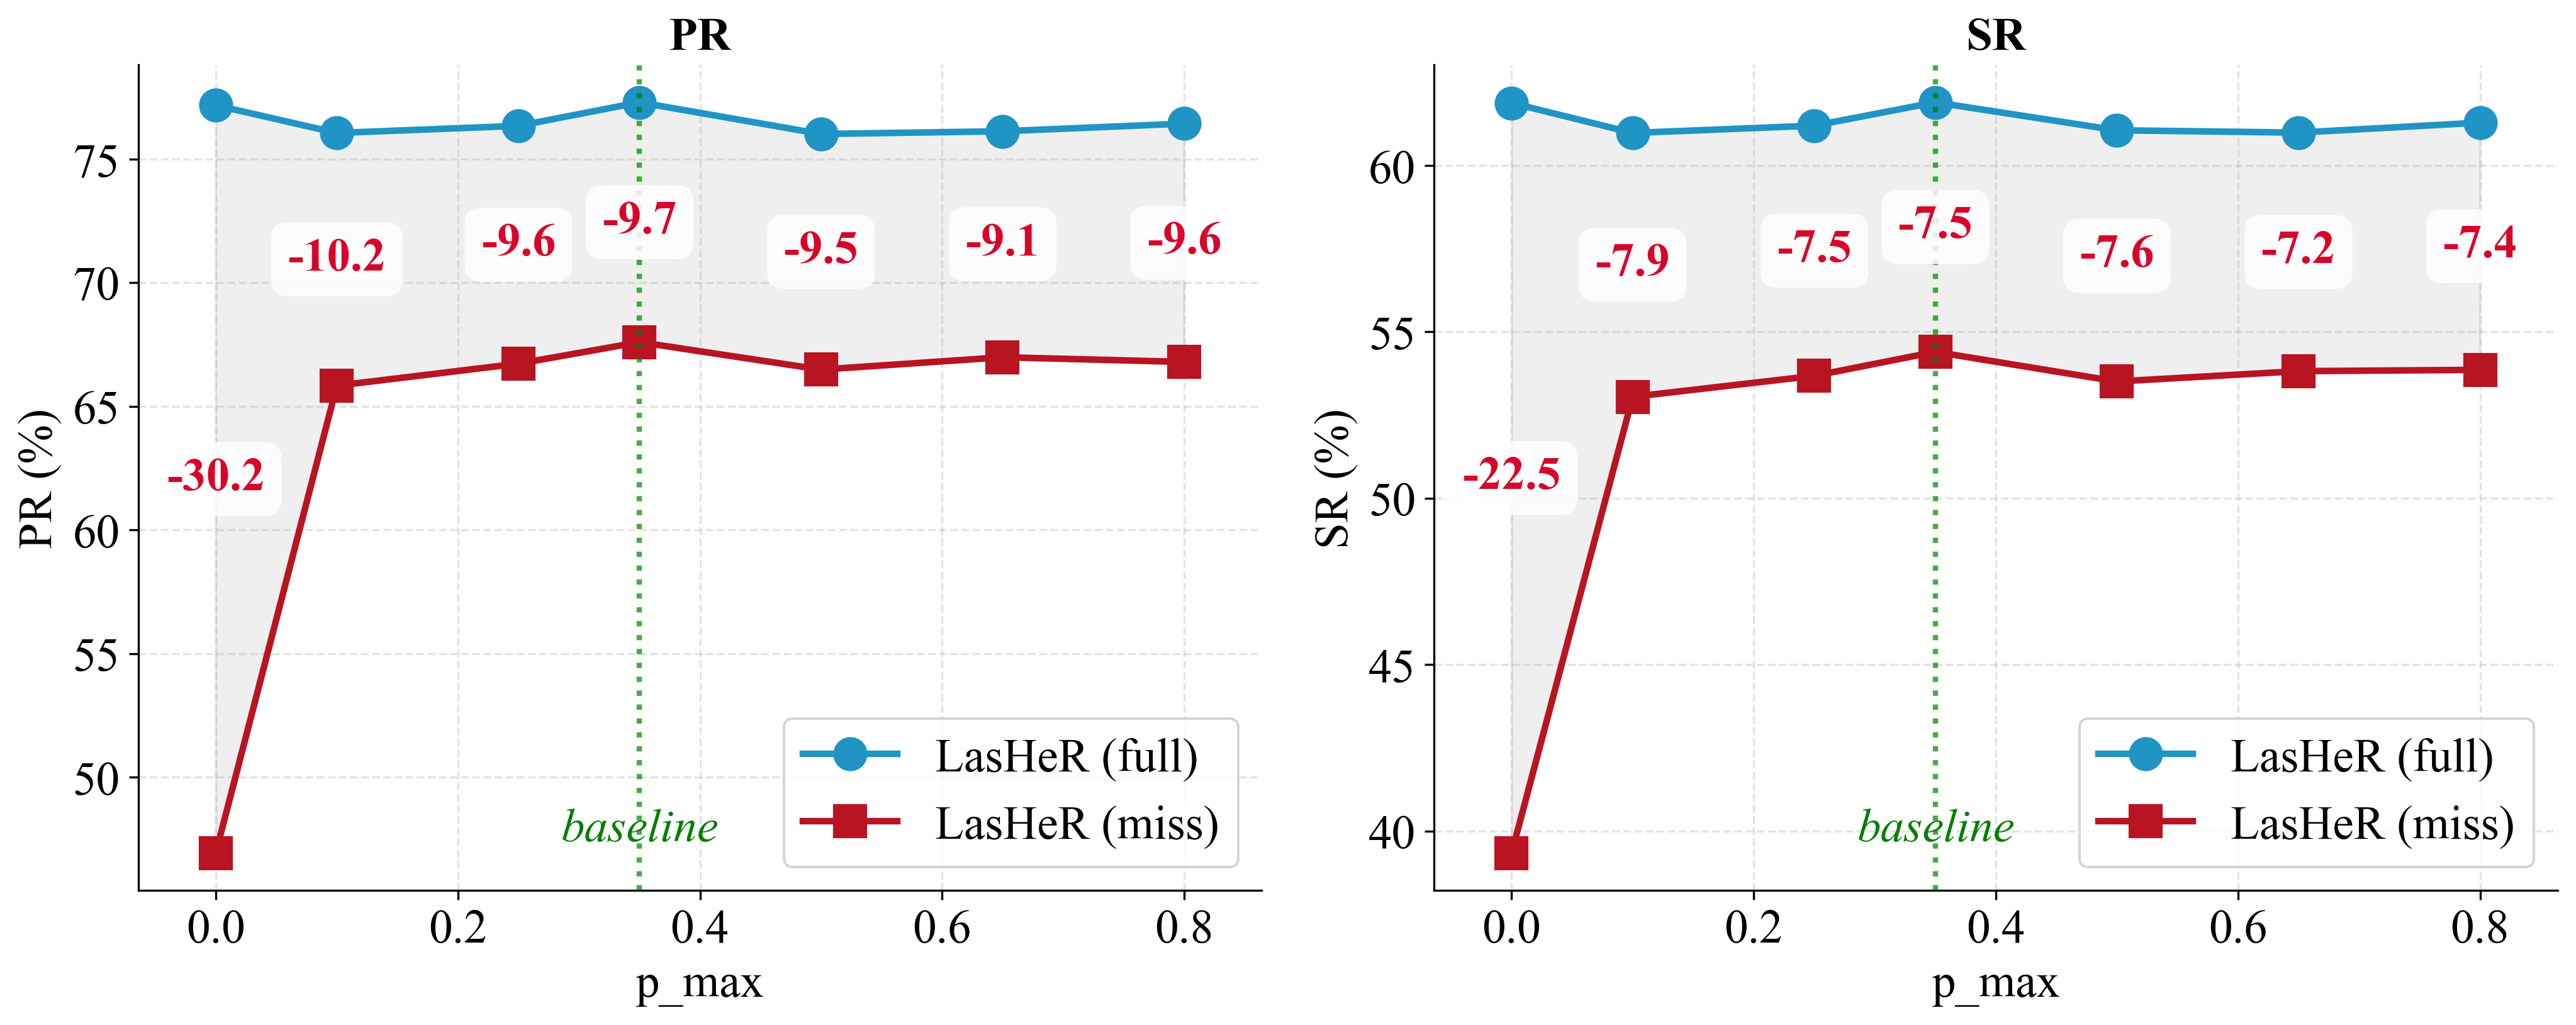
\includegraphics[width=\linewidth]{figures/line_pmax.png}
    \caption{Sensitive analysis for $p_{\text{max}}$ on LasHeR}
    \label{fig-ablation_cma}
\end{figure}

\paragraph*{Heterogeneous vs. Homogeneous Experts}
\begin{table}[ht]
\caption{Comparison between heterogeneous and homogeneous experts on DepthTrack.}
\label{tab:ablation_moe}
\centering
\small
\begin{tabular}{cc|ccc}
\toprule
Type & Config & F-Score & Re & Pr \\
\midrule
\multirow{3}{*}{Hom. Experts} & small & 55.6 & 56.8 & 54.4 \\
 & middle & 56.0 & 57.2 & 54.7 \\
 & large &  &  &  \\
\midrule
\multirow{2}{*}{Het. Experts} & hybrid & 57.5 & 58.8 & 56.2 \\
& \textbf{Ours} & \textbf{58.8} & \textbf{60.1} & \textbf{57.5} \\
\bottomrule
\end{tabular}
\end{table}

We further compare homogeneous and heterogeneous experts on the DepthTrack benchmark, as illustrated in Tab. \ref{tab:ablation_moe}. Specifically, we evaluate MoE models with different expert capacities by setting the hidden width to 4, 32, and 512 for the small, medium, and large configurations, respectively, as well as a straightforward Vanilla Hybrid MoE architecture. The results reveal that, for homogeneous-expert models, increasing the expert capacity consistently improves tracking performance (55.6 $\rightarrow$ 56.0 $\rightarrow$ XXX for F-score); however, their performance remains inferior to that of heterogeneous-expert models. For heterogeneous-expert models, the Vanilla Hybrid MoE consistently underperforms our proposed HMoE under comparable model capacities (57.5 / 58.8 / 56.2 v.s. 58.8 / 60.1 / 57.5 for F-score, Recall and Precision).

These findings demonstrate that \textit{the performance gains of HMoE stem from capacity diversity rather than the overall model capacity.} Specifically, modality missing leads to inefficient utilization of computational resources in homogeneous-expert architectures, while a naive hybrid design lacks the flexibility to allocate computational capacity according to the input characteristics. In contrast, the proposed heterogeneous-expert architecture can adaptively adjust expert capacity based on the availability of modality information, thereby maximizing the utilization of existing computational resources.

\subsection{Qualitative Results}
% \label{subsec:qualitative}
% % Add a paragraph referencing your visual tracking results figure.
% Figure~\ref{fig:qualitative} visualizes tracking results under severe modality dropout. When the thermal camera stalls (e.g., crossing a cold background), baseline methods lose the target entirely. FlexTrack-V2 successfully hallucinates the missing thermal contours from the RGB stream, retaining a tight bounding box on the target.
